\documentclass{beamer}
\usetheme{Goettingen}

\usepackage{amsmath}
\usepackage{fontspec}
\usepackage{unicode-math}
\usepackage{graphicx}

% --- TikZ ---
\usepackage{adjustbox}
\usepackage{tikz}

\usetikzlibrary{math, shapes, arrows}

\tikzstyle{terminator} = [
  rectangle,
  draw,
  text centered,
  rounded corners,
  minimum height=2em
]

\tikzstyle{data} = [
  trapezium,
  draw,
  text centered,
  trapezium left angle=60,
  trapezium right angle=120,
  minimum height=2em
]

\tikzstyle{team} = [rectangle, draw, text centered, minimum height=2em]

\tikzstyle{connector} = [draw, -latex']

% --- Listings ---
\usepackage{listings}

\lstset{language=Python,
  basicstyle=\ttfamily\footnotesize,
  keywordstyle=\color{magenta}
}

% --- Hyperlinks ---
\usepackage{hyperref}

\hypersetup{
  colorlinks=true,
  linkcolor=blue,
  filecolor=magenta,
  urlcolor=cyan,
  pdftitle={Rocket Calculator},
  pdfpagemode=FullScreen
}

% --- Fonts ---
\setmainfont{DejaVu Sans Mono}
\setmathfont{Concrete Math}
\setmonofont{Iosevka}

%\setlist[itemize]{label=--}

\newcommand{\diff}[1]{\ensuremath{\mathop{}\!\mathrm{d}}#1}
\newcommand{\ndiff}[2]{\ensuremath{\mathop{}\!\mathrm{d}^{#1}}#2}

\title{A Sufficiently Generic Rocket Calculator}
\date{\today}

\begin{document}

\begin{frame}
  \titlepage
\end{frame}

\begin{frame}{Outline}
  \tableofcontents
\end{frame}

\section{Problem statement}
\begin{frame}{Hybrid engine rocket}
  \centering
  \includegraphics[width=\columnwidth]{../notes/fig/Hybrid-rocket-engine.jpg}
\end{frame}

\begin{frame}{Data flow}
  \centering
  \begin{adjustbox}{max width=\textwidth, max height=.7\textheight}
  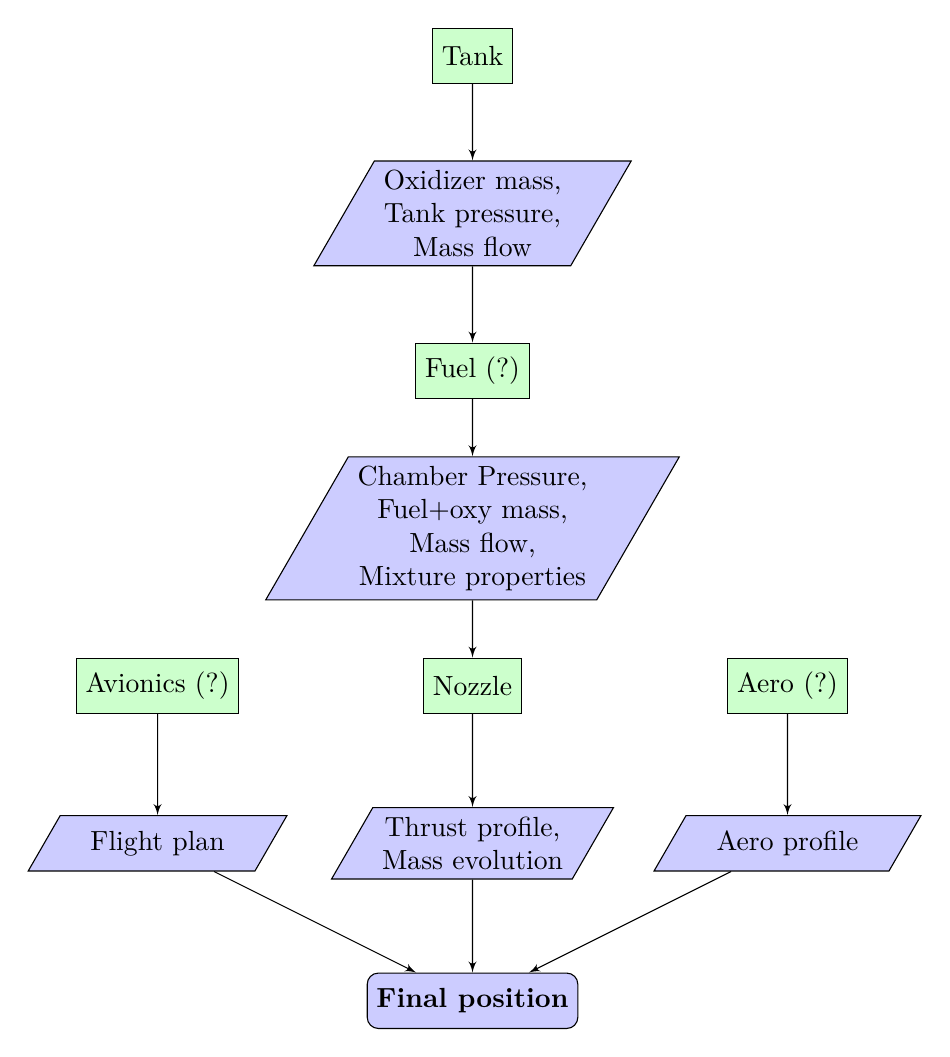
\begin{tikzpicture}
    \pgfmathsetmacro{\hsp}{4}
    \pgfmathsetmacro{\vsp}{2}

    \node [terminator, fill=blue!20] at (0,0) (position)
      {\textbf{Final position}};

    % --- Aerodynamics branch ---
    \node [data,  fill=blue!20] at (\hsp,   \vsp) (aero)  {Aero profile};

    \node [team, fill=green!20] at (\hsp, 2*\vsp) (aero_t) {Aero (?)};

    % --- Flight plan/avionics branch ---
    \node [data,  fill=blue!20] at (-\hsp,   \vsp) (attitude) {Flight plan};

    \node [team, fill=green!20] at (-\hsp, 2*\vsp) (avionics) {Avionics (?)};

    % --- Propulsion branch ---
    \node [data, fill=blue!20, align=center] at (0, \vsp) (thrust)
      {Thrust profile,\\Mass evolution};

    \node [team, fill=green!20] at (0, 2*\vsp) (nozzle) {Nozzle};

    \node [data, fill=blue!20, align=center] at (0, 3*\vsp) (chamber)
      {Chamber Pressure,\\Fuel+oxy mass,\\Mass flow,\\Mixture properties};

    \node [team, fill=green!20] at (0, 4*\vsp) (fuel) {Fuel (?)};

    \node [data, fill=blue!20, align=center] at (0, 5*\vsp) (injector)
      {Oxidizer mass,\\Tank pressure,\\Mass flow};

    \node [team, fill=green!20] at (0, 6*\vsp) (tank) {Tank};

    \path [connector] (aero)     -- (position);
    \path [connector] (thrust)   -- (position);
    \path [connector] (attitude) -- (position);

    \path [connector] (avionics) -- (attitude);

    \path [connector] (aero_t)   -- (aero);

    \path [connector] (nozzle)   -- (thrust);
    \path [connector] (chamber)  -- (nozzle);
    \path [connector] (fuel)     -- (chamber);
    \path [connector] (injector) -- (fuel);
    \path [connector] (tank)     -- (injector);
  \end{tikzpicture}
  \end{adjustbox}
\end{frame}

\section{Program components}

\subsection{Flight plan}
\begin{frame}[fragile]{Attitude}
  $\mathbf x$ - position relative to launch site, \\
  $\mathbf v$ - velocity relative to launch site

  \vspace{\baselineskip}

  Attitude as a lookup table:

  \begin{equation}
    \mathcal A:
    \begin{aligned}[t]
      \mathbb R^3, \mathbb R^3
      & \to \mathbb R^3 \text{ (or $\mathbb H$)} \\
    \mathbf x, \mathbf v & \mapsto (\phi, \theta, \psi)
    \end{aligned}
  \end{equation}

  \vspace{\baselineskip}

  \begin{lstlisting}
  Array3D = np.typing.NDArray[np.float64]

  def attitude(x: Array3D, v: Array3D) -> Array3D: ...
  \end{lstlisting}
\end{frame}

\subsection{Aerodynamics}
\begin{frame}[fragile]{Aerodynamics}
  Atmospheric conditions table:

  \begin{equation}
    \mathbf A:
    \begin{aligned}[t]
      \mathbb R^3 & \to \mathbb R, \mathbb R, \mathbb R, ... \\
      \mathbf x & \mapsto (P_\text{atm}, T_\text{atm}, w, \ldots)
    \end{aligned}
  \end{equation}

  \vspace{\baselineskip}

  Drag profile (dimensionless):

  \begin{equation}
    C_\text{D}:
    \begin{aligned}[t]
      \mathbb R^3, \mathbb R^3, \mathbb R^3 & \to \mathbb R \\
      \mathbf x, \mathbf v, \mathcal A & \mapsto C_\text{D}
    \end{aligned}
  \end{equation}

  (neglect attitude assuming rocket is aligned with velocity vector)

  \vspace{\baselineskip}

  \begin{lstlisting}
  def drag(x: Array3D, v: Array3D) -> np.float64: ...
  \end{lstlisting}

  Depends on the shape of the rocket
\end{frame}

\subsection{Propulsion}

\subsubsection{Nozzle}
\begin{frame}{Nozzle thrust profile}
  Thrust profile:
%
  \begin{equation}
    F_\text{T,e} = F_\text{T,e} (t)
  \end{equation}
%
  Ideally, the engine thrust depends on the mass flow, exit velocity, exit
  pressure and nozzle exit cross-section:
%
  \begin{equation}
    F_\text{T,e} (t) = \dot m(t) u_\text{e} (t) + P_\text{e} (t) A_\text{e}
  \end{equation}
%
  Real thrust is then the engine thrust adjusted for atmospheric conditions,
  efficiency, and drag:
%
  \begin{alignat}{2}
    F_\text{T}
    & = F_\text{T,e} \cdot \eta
      - P_\text{amb} \cdot A_\text{e}
      - F_\text{D} \nonumber\\
    & = (\dot m u_\text{e} + P_\text{e} A_\text{e}) \cdot \eta
      - P_\text{amb} A_\text{e} - F_\text{D}
  \end{alignat}
%
  $\eta$ is the efficiency parameter that depends on the nozzle shape
\end{frame}

\begin{frame}{Typical convergent-divergent nozzle}
  \centering
  \includegraphics[width=\columnwidth]{
    ../notes/fig/convergent-divergent-nozzle.png
  }
\end{frame}

\begin{frame}{Parabolic nozzle}
  \centering
  \includegraphics[width=\columnwidth]{../notes/fig/parabolic-nozzle.jpeg}
\end{frame}

\begin{frame}{Nozzle efficiency}
  $z$ - axial position with nozzle entrance ("chamber") at $z = 0$

  \vspace{\baselineskip}

  Then, model nozzle shape as some form-factor function $f(z)$

  \vspace{\baselineskip}

  Nozzle efficiency is a function of this form-factor, $\eta[f(z)]$

  \vspace{\baselineskip}

  Need simulations to determine exactly:

  \begin{itemize}
  \item[--] \texttt{NozzleMate}: a Python solution
  \item[--] further options?
  \end{itemize}
\end{frame}

\subsubsection{Chemistry with CEA}
\begin{frame}{Thrust calculations}
  \begin{equation*}
    \dot{m} = \frac{P_\text{c} A_\text{t}}{c^*}
  \end{equation*}

  where $P_\text{c}$ is the chamber pressure and $c^*$ is the
  \emph{characteristic velocity} computed with CEA.

  \vspace{\baselineskip}

  Engine thrust:

  \begin{equation*}
    F_\text{T,e}
    = \dot{m} I_\text{sp} g_0
    = C_\text{f} A_\text{t} P
  \end{equation*}

  compute with $I_\text{sp}$ or $C_\text{f}$ (\emph{thrust coefficient})
  provided by CEA.
\end{frame}

\begin{frame}[fragile]{Thrust profile inputs}
  Engine thrust:

  \begin{equation}
    F_\text{T} (t)
    = F_\text{T} [\dot m(t), u_\text{e}(t), P_\text{e}(t), A_\text{e}]
  \end{equation}

  We calculate all of these using the CEA library

  \vspace{\baselineskip}

  Real thrust accounting for efficiency and atmospheric conditions:

  \begin{equation}
    F_\text{T} (t)
    = F_\text{T} [
      \dot m(t), u_\text{e}(t), P_\text{e}(t), A_\text{e};
      \eta, \mathbf A
    ]
  \end{equation}
\end{frame}

\begin{frame}[fragile]{CEA solver}
  \begin{lstlisting}[basicstyle=\ttfamily\tiny]
  mixture = [
      {
          name: "H2(L)", temp: 20.27,
          fraction: 1.0, fuel_weight: 1.0, oxidant_weight: 0.0
      },
      {
          name: "O2(L)", temp: 90.17,
          fraction: 1.0, fuel_weight: 0.0, oxidant_weight: 1.0
      }
  ]
  \end{lstlisting}

  Isolating the essential arguments of the CEA rocket solver, one can define a
  function of the following form:

  \begin{lstlisting}[basicstyle=\ttfamily\tiny]
  def solve(
      mixture : dict,             # mixture component dictionary
      pc      : np.float64,       # chamber pressure
      subar   : list[np.float64], # subsonic area ratio
      supar   : list[np.float64]  # supersonic area ratio
  ) -> cea.RocketSolution:

      ... # implementation details

      solver.solve(solution, weights, pc, pi_p, subar=subar, supar=supar, hc)

      return solution.c_star, solution.Cf
  \end{lstlisting}
\end{frame}

\end{document}

